\documentclass[11pt, titlepage, oneside]{article}

\usepackage{caption}
\usepackage{float}
\usepackage{times}
\usepackage[margin = 2cm]{geometry}
\usepackage{graphicx}
\usepackage{amssymb}
\usepackage{amsmath}
\usepackage{amsthm}
\usepackage{natbib}
\usepackage{epstopdf}
\usepackage{enumerate}
\usepackage{url}
\usepackage{todonotes}
\usepackage{mdwlist} 						%% Compact lists 
\usepackage{tikz}							%% Uncomment if you're using diagrams
\usepackage{pgfgantt}
\geometry{a4paper}
%\linespread{1.6}							%% Increase or decrease line spacing

% Proof Style
\renewcommand{\qedsymbol}{$\blacksquare$} 	%% Ends proofs with a black square, comment out for the standard box

% Theorem Styles
\theoremstyle{plain}
\newtheorem{theorem}{Theorem}[section]
\newtheorem{lemma}{Lemma}[theorem]
\newtheorem{proposition}{Proposition}[theorem]
\newtheorem{corollary}{Corollary}[theorem]

\theoremstyle{definition}
\newtheorem{definition}{Definition}[section]
\newtheorem{fact}{Fact}

\theoremstyle{remark}
\newtheorem{exercise}{Exercise}[section]
\newtheorem{example}[exercise]{Example}
	
%% Most people number theorems,lemma & propositions together
%% and wouldn't number a definition

% List Styles
\renewcommand{\theenumi}{\roman{enumi}}   	%% Choose to uncomment this
%\renewcommand{\theenumi}{arabic}  			%% Or this
\pagenumbering{arabic}

%relative image paths and image file types
%\DeclareGraphicsExtensions{.pdf,.png,.jpg,.eps}
\graphicspath{ {./images/} }

% Title and Author of the document
\title{Automatic classification of fossils and insects}
\author{Matthew Lee}
\date{\today}                						

\begin{document}
%\pdfximage width 0.3\textwidth {Argynnis-aglaja-02.png}
%\edef\imgi{\pdfrefximage\the\pdflastximage\relax}
%\pdfximage width 0.3\textwidth {Aglais-urticae-02.png} 
%\edef\imgii{\pdfrefximage\the\pdflastximage\relax}

\begin{minipage}[b]{\linewidth}
	\center
	\textsc{\Large Automatic classification of fossils and insects}\\
	\vspace{1.0cm}
	\Large Literature Survey \\
	\vspace{1.0cm}
	\normalsize Matthew Lee\\
	\normalsize \texttt{matthew.lee13@imperial.ac.uk}\\
	\normalsize Supervised by Doctor Benjamin Glocker\\
	\vspace{0.35cm}
\today
\end{minipage}

\hspace{0.375cm}

\tableofcontents

%% =======================================================================%%
%%                                                                              Introduction
%% =======================================================================%%
\newpage
\section{Introduction}
	Swedish botanist Carolus Linnaeus, often referred to as the father of taxonomy, developed the system known today as Linnaean classification for the categorisation of organisms  based on morphology in the 18th century. Though taxonomy has come a long way since then, and is now based on evolutionary relationships between organisms, identification by morphological traits is still very common. Qualitative descriptions of features, coupled with subjective analysis of organisms, can lead to erroneous classifications\cite[p.~154]{nature} which emphasises the need for a more quantitative approach. The goal of the project is to develop software which is capable of autonomously identifying different species of butterflies using feature detection. The difficulty in such a task lies in the intra species dissimilarity and the inter species similarity (see figure \ref{fig:difference}), we will be working with a data set consisting of 57 different species of butterfly, each with 5 to 10 images. \\

		\begin{figure}[H]
			\centering
			\begin{tabular}{cc}
				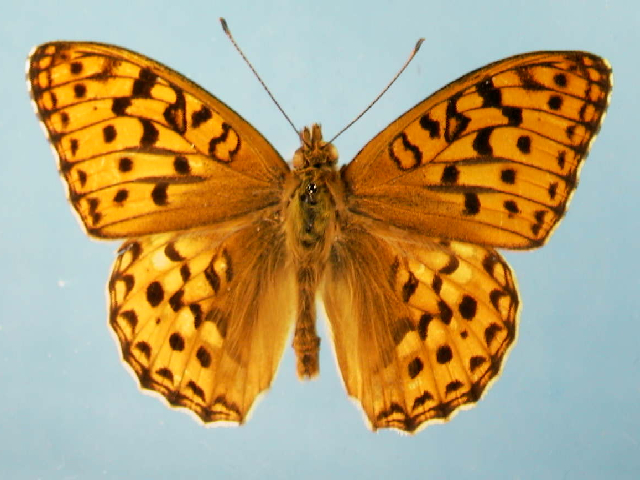
\includegraphics[width=0.4\textwidth]{Argynnis-adippe-05.jpg} &
				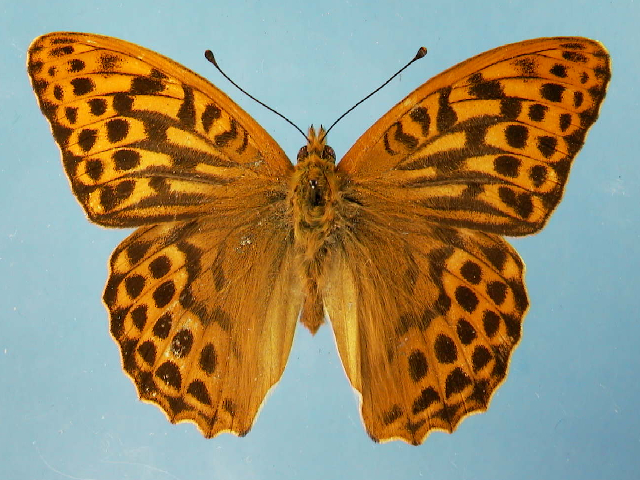
\includegraphics[width=0.4\textwidth]{Argynnis-paphia-05.jpg} \\
				Argynnis-adippe & Argynnis-paphia \\
				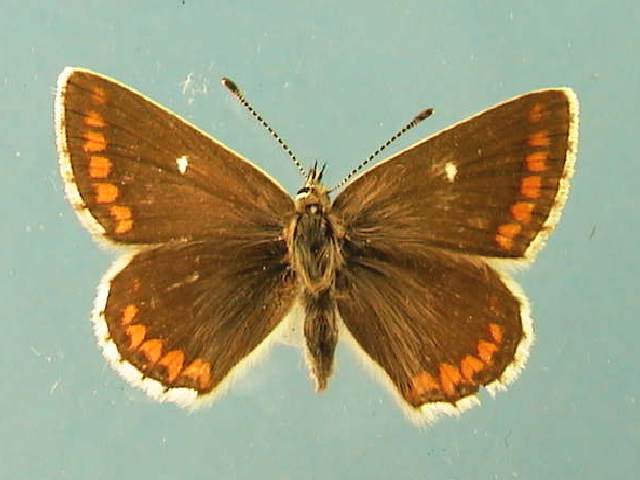
\includegraphics[width=0.4\textwidth]{Aricia-artaxerxes-08.jpg}&
				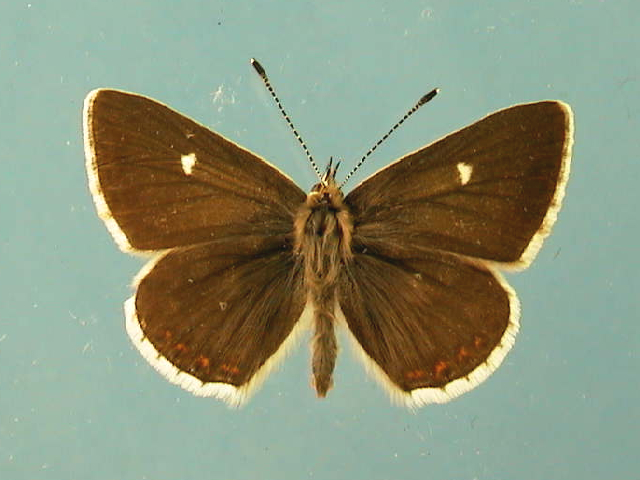
\includegraphics[width=0.4\textwidth]{Aricia-artaxerxes-05.jpg}\\
				Aricia-artaxerxes & Aricia-artaxerxes
			\end{tabular}
			\caption{A demonstration of intra species dissimilarity and inter species similarity}
			\label{fig:difference}
		\end{figure}	

	\noindent The Natural History Museum currently has DAISY (Digital Automated Identification System), trained on the same image set, it has a successful identification rate of 91.4\%\cite{overview}. DAISY makes use of plastic self organising maps (see section \ref{subsec:psom}), meaning the system is efficient and quick to retrain when additions to the training set are made. However the main drawback of the system is that a user must manually outline the wings of the butterflies in an image before the butterfly can be categorised. This project will look to achieve similar rates of successful identification in a fully automated manner, if realised this would mark a vast improvement in the current technology\cite{DAISY}. \\

	\noindent Given that similar existing software requires human interaction such as outlining the wing of a moth\cite{book} and that co-segmentation as a stage of data processing has already been shown to improve visual recognition\cite{vis}, there will need to be a preprocessing stage that is capable of highlighting the butterfly from the background. In addition since redundant class specific information is present in our particular data set, it will serve to prevent any feature detectors from learning afore mentioned features. For example all Aglais Urticae have been preprocessed and a black background has been applied, whereas all Argunnis Aglaja have blue backgrounds (see figure \ref{fig:background}). Hence there will  be three major sections of the software, which will be developed as separate modules, a segmentation module, a classification module and the user interface.
		
		\begin{figure}[H]
			\centering
			\begin{tabular}{cc}
			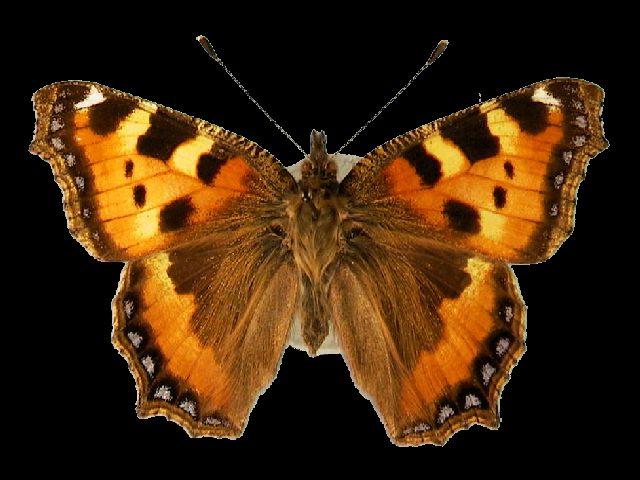
\includegraphics[width=0.4\textwidth]{Aglais-urticae-02.jpg} &
			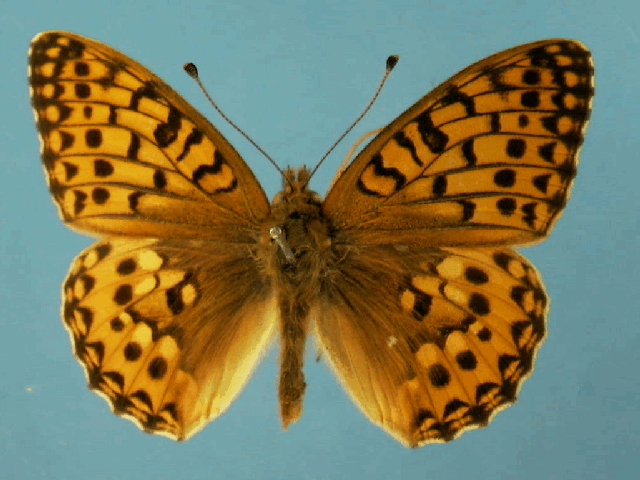
\includegraphics[width=0.4\textwidth]{Argynnis-aglaja-02.jpg}
			\end{tabular} 
			\caption{Comparison of two species of butterflies that can be distinguished by their background colours}
			\label{fig:background}
		\end{figure}
	
%% =======================================================================%%
%%                                                                              Methodology
%% =======================================================================%%

\section{Methodology}
	\subsection{Segmentation}
		Segmentation is the separation of the foreground objects from the background: outlined below are a number of segmentation methods used for improving classification error of images.
		
		\subsubsection{Interactive Graph Cuts}
			The use of an interactive graph cutting\cite{ND} to segment objects from their background has proven successful in improving the accuracy of classification algorithms\cite{vocab}. This could be automated by using predefined anchor points for foreground and background markers, such anchor points could be found analytically by first manually finding foreground regions for a set of training data $\{T^{f}_1,...,T^{f}_N\}$ and simply overlaying all training images, finding the the intersection of all foreground regions $T^{f}_{\text{common}} := \bigcap_{1}^{N}T^{f}_n$. Similarly safe background anchor points can be found.
	
		\subsubsection{GrabCut}
			In the paper \emph{Recognition between a Large Number of Flower Species}\cite{chai} a fast and accurate procedure known as GrabCut\cite{grabcut} is used as part of the image segmentation pipeline. The procedure is iterative and segments by energy minimisation. The algorithm requires user input in the form of a bounding box, this specifies the definite background region $T_B$. $T_U$, the unknown region, is set to $T_B^{\mathsf{c}}$ and $T_F$ the foreground is found. However if a data set is consistent enough it is possible to use the same bounding box on all images in order to fully automate the process. 
		%%% NOT SURE IF THIS SHOULD BE INCLUDED, SEEMS A BIT TOO DETAILED
		%%%
			\iffalse
			The GrabCut\cite{grabcut} algorithm uses a manually set bounding box that separates foreground from background. Given this box the GrabCut algorithm segments the foreground object using the following is a summary of the procedure (taken from \cite{grabcut} with additional annotations):
			\begin{itemize}
				\item Given a trimap $T$, let an image be represented by the vector $(z_1,...,z_N)$ in RGB colour space. Segmentation described by $\underline{\alpha}$ values $(\alpha_1,...,\alpha_N)$ where $\alpha_n \in \{0,1\}$ $1$ if the pixel is in the foreground and $0$ if it part of the background. Two full covariance gaussian mixture models with $K$ components are found, one for the background. Let $\mathbf{k} = (k_1,...,k_n)$ where $k_n\in \{1,...K\}$ assigns each pixel a GMM component, either from the foreground or background model (in accordance to $\alpha_n$ value).
				\item let $\underline{\theta}$ describe the greyscale histogram for the foreground and background, normalised such that $\int_{\mathbf{z}} h(\mathbf{z};\mathbf{\alpha}) = 1$
					\[
						\underline{\theta} = \{h(\mathbf{z};\mathbf{\alpha}), \alpha = 0,1 \}
					\]
				\item Define 
					\[
						f
					\]
				\item Initialise trimap $T$ by supplying only $T_B$ the foreground is set to $T_F = \emptyset$; $T_U = T_B^{\mathsf{C}}$, complement of the background.
				\item Initialise $\alpha_n = 0$ for $n \in T_B$ and $\alpha_n = 1$ for $n \in T_U$
				\item Background and foreground gaussian mixture models (GMM) initialised from sets $\alpha_n = 0$ and $\alpha_n = 1$ respectively
			\end{itemize}
			\textbf{Iterative Minimisation}
			\begin{enumerate}
				
				\item Assign GMM components to pixels: for each $n$ in $T_U$
					\[
						k_n := \arg \min_{k_n} D_n (\alpha_n,k_n, \theta, z_n)
					\]
				\item Learn GMM parameters from data $\mathbf{z}$:
					\[
						\underline{\theta} := \arg \min_{\underline{\theta}} U(\underline{\alpha}, \mathbf{k}, \underline{\theta}, \mathbf{z})
					\]
				\item Estimate segmentation: use min cut to solve:
					\[
						\min_{\alpha_n: n\in T_U} \min_{\mathbf{k}} \mathbf{E}(\underline{\alpha}, \mathbf{k}, \underline{\theta}, \mathbf{z})
					\]
				\item Repeat from step 1, until convergence
				\item Apply border matting
				
			\end{enumerate}
			 This reduces the input required from the user and given the standard format of the image set is suitable for the task. However, future iterations of the software may wish for this to be changed and implemented with user interaction for more accurate segmenting.
			 \fi
			 %%%
			 %%% END OF COMMENT
		\subsubsection{BiCos Approach}
			Advancements on the GrabCut\cite{grabcut} algorithm have recently been made, namely the Bi-level Co-Segmentation\cite{bicos} algorithm, as used by the Oxford visual geometry group\cite{robot} in the classification of 102 flower species trained on 20 images per class (Oxford 102 dataset \cite{oxford102}). The procedure builds on top of the GrabCut procedure by using it to obtain an initial label for super pixels, obtained by  splitting the image into segments using a graph-based approach\cite{felz}. With each segment a description vector is created using 5 sub-metrics (colour distribution, SIFT\cite{sift} distribution, size, location within the image and shape). This information is then passed through a support vector machine and a hyperplane in the description space is found which separates the segments and any incorrect labels are adjusted according to hyperplane. This hyperplane can then be used to find a saliency map for an image and a graph-cut algorithm used to separate the foreground and background.

		\subsubsection{Other Considerations}
			\begin{itemize}
				\item \textbf{Region Growing}. Given that the background of our sample images are plain compared to our foreground, one approach could be the use of  manually anchoring seeding points around the peripheral of the image and using a region growing algorithm. Once the algorithm has connected our background points into a single region we can take the inverse of the region to be our foreground. We use the background as our seed point as given the complexity of colour of the subject it could take many iterations before the foreground is ever fully connected, more dangerously the entire background could have been incorporated before the butterfly. 
				\item \textbf{K-means Clustering}. Using a K-means clustering style approach we can define peripheral regions $X_1,...,X_n$ with initial interior points $x_1,..., x_n$ which are manually anchored. Growing each region $i$ by adding adjacent pixels $y_1,...,y_m$ if $|m_i - y_j| < \delta$ where $\displaystyle m_i = \frac{\sum\limits_{e_k \in X_i} e_k}{|X_i|}$ represents the region mean according to a metric $e_k$ for each pixel such as intensity, RGB value or perhaps grey scale. $\delta$ would be experimentally obtained and represents a growth rate for a region.
			\end{itemize} 

	\subsection{Classification}
		The classification of images has been approached many times in many different ways, an analysis of experiments using different techniques and a brief description of the data sets involved in the training process follow.


		\subsubsection{Convolutional Neural Networks}
			Given larger data sets such as the ImageNet LSVRC2010 contest which has 1.2 million images containing 1000 classes\cite{imagenetsite}, competitors\cite{imagenet} used deep convolutional neural networks with a successful classification rate of 37.5\%. The advantage of using a convolutional neural network is the autonomy of feature learning. With the focus of taxonomy in mind, it would be an interesting experiment to see if the statistically learnt features couple well with the morphological descriptions given by taxonomists. \\
			
			\noindent\textbf{Dropout}\cite{dropout}. Dropout is a recent development in convolutional neural networks which helps prevent over fitting. During the training of the network the output of a neuron is  set to $0$ with probability half, its weights and bias are also not updated if this occurs for the neuron. The aim is to have the remaining neurons detect meaningful features independent of the neurons that have been `dropped out'. This reduces the amount of advanced co dependency within the network. Though this leads to an increase in training time it has been advantageous in substantially reducing over fitting\cite{imagenet}.
			
		%\subsubsection{Deep Fischer Networks}
		\subsubsection{Plastic Self Organising Maps}
			\label{subsec:psom}
			A self organising map is a special type of neural network, neurons here store weight vectors and are arranged in a grid (see figure \ref{fig:som}). These weights are the same dimensionality as the input space and represent some cluster of input values. The neurons are intialised with random weights and when presented with training data the nearest neuron is found and adjusted to better represent the training example by some predefined learning rate. Neurons which are close together in this gridded structure can affect each other, i.e. when a neuron is updated (its weights changed) its neighbours will also be changed, however neurons which are far away will not affect each other. DAISY uses an adaptation of this method\cite{science,dice}, plastic self organising maps. In these neural networks rather then arranging neurons in a fixed grid, they are given relative distances to each other that can be updated (see figure \ref{fig:psom}), note also that if this distance grows too large the relation can be broken.\\

			\begin{figure}[H]
				\centering
				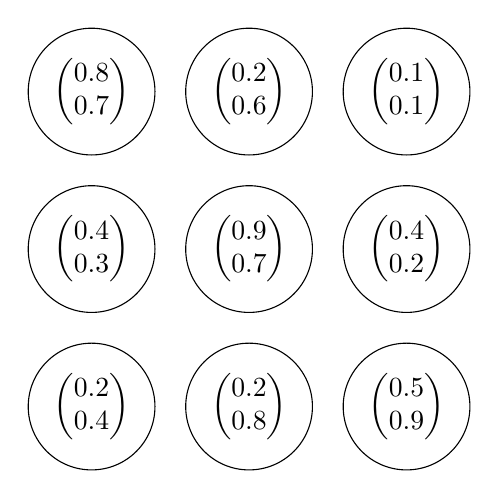
\begin{tikzpicture}
					\node[draw, circle] at (0,0){$\begin{pmatrix}0.2\\0.4\end{pmatrix}$};
					\node[draw, circle] at (0,2){$\begin{pmatrix}0.4\\0.3\end{pmatrix}$};
					\node[draw, circle] at (0,4){$\begin{pmatrix}0.8\\0.7\end{pmatrix}$};
					\node[draw, circle] at (2,0){$\begin{pmatrix}0.2\\0.8\end{pmatrix}$};
					\node[draw, circle] at (2,2){$\begin{pmatrix}0.9\\0.7\end{pmatrix}$};
					\node[draw, circle] at (2,4){$\begin{pmatrix}0.2\\0.6\end{pmatrix}$};
					\node[draw, circle] at (4,0){$\begin{pmatrix}0.5\\0.9\end{pmatrix}$};
					\node[draw, circle] at (4,2){$\begin{pmatrix}0.4\\0.2\end{pmatrix}$};
					\node[draw, circle] at (4,4){$\begin{pmatrix}0.1\\0.1\end{pmatrix}$};
				\end{tikzpicture}
				\caption{simple example of a self organising map, where intial weights have been set randomly}
				\label{fig:som}
			\end{figure}

			\begin{figure}[H]
				\centering
				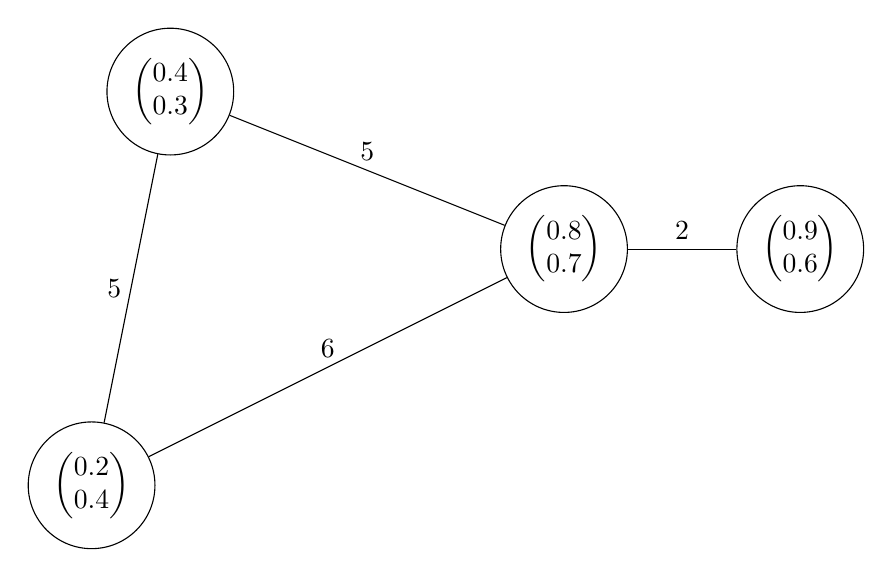
\begin{tikzpicture}
					\node[draw, circle] at (0,0)(a){$\begin{pmatrix}0.2\\0.4\end{pmatrix}$};
					\node[draw, circle] at (1,5)(b){$\begin{pmatrix}0.4\\0.3\end{pmatrix}$};
					\node[draw, circle] at (6,3)(c){$\begin{pmatrix}0.8\\0.7\end{pmatrix}$};
					\node[draw, circle] at (9,3)(d){$\begin{pmatrix}0.9\\0.6\end{pmatrix}$};
					\draw (a)edge node[left]{5}(b);
					\draw (a)edge node[above]{6}(c);
					\draw (b)edge node[above]{5}(c);
					\draw (c)edge node[above]{2}(d);
				\end{tikzpicture}
				\caption{simple example of a plastic self organising map, where intial weights have been set randomly}
				\label{fig:psom}
			\end{figure}
			
		\subsubsection{$k$-Nearest Neighbours}
			The $k$-Nearest Neighbour classification procedure is simple to implement and quick to retrain. Given some training set $(\mathbf{x}_1,y_1),...,(\mathbf{x}_n,y_n)$ where $\mathbf{x}_i \in \mathbb{R}^{d}$ and $y_i \in \{1,...,p\}$ are representative of our classes, the problem of classifying a new point $\mathbf{v} \in \mathbb{R}^d$ as belonging to a class is reduced to finding the $k$ nearest elements from our training set and finding the majority vote of $y_i$'s, the class values for each of the $k$ neighbours. Note that by nearest we have assumed the use of some metric $d(\cdot,\cdot)$ in our input space. Previous iterations of DAISY have used a variant of k-nearest neighbour classification\cite{DAISY,book} known as Lucas $n$-tuple nearest neighbour classification\cite{lucas} where the $d$ dimensional input space is broken into $m$ $n$-tuples, that is the input vector $\mathbf{x}=(x_1,...,x_d)$ is projected into $m$ elements $\mathbf{y}_j = (x_{a_{j1}},...,x_{a_{jn}})$ which exist in $n$-dimensional space. we will denote the $k$th vector of the $n$-tuple $j$ for the $c$th class as $\mathbf{y}_{jk}^c$. Training is then just the process of breaking down our training input into these sub sampled vectors. Classification works in a similar way to \emph{kNN}, given some new vector $\mathbf{z}$ we assign a classification score $r_c$ to class $c$ as follows:
			\[
				r_c = \sum_{j=1}^{m}\arg\min_k d(\mathbf{y}_{jk}^c,z_j)
			\]
		The classification is then defined as $v$ such that $r_v$ is the minimum over all classes. Previous iterations of DAISY have used nearest neighbour classification algorithms using the normalised vector distance (NVD) metric\cite[p.~104]{book} where $d(\mathbf{x},\mathbf{y}):= \sum_{}|x_{i}^{2}-y_{i}^{2}|$.

		\subsubsection{Bag of Words}
			Nilsback et al\cite{vis}. use a bag of words approach to classify 17 flower species with 80 training images per species. This method breaks features into three groups; colour, shape and texture, each represented with a vector which they eventually combine and pass through a non linear support vector machine. An image is broken into $n$ super pixels using k-means clustering, the colour of the image is then represented by an $n$ dimensional normalised frequency histogram. Shape is represented using SIFT\cite{sift} descriptors optimised over a grid. To quantise texture Nilsback et al. convolve the image using the rotation invariant MR8 filter bank\cite{mr8}. If similar `texture' properties that are not invariant to rotation need to be extracted from an image another filter bank could be used, alternatively the MR8 filter bank could be used without the maximum response function. \\
			
			\noindent Lazebnk et al\cite{pyramid}. introduced an enhancement to this technique, spatial pyramids. By partitioning the image into subregions and performing a bag of words analysis on the subregions, repeating with ever finer subregions we are able to preserve some global locational information. Subregion $0$ is defined as the whole image, at level $k+1$ each dimension at level $k$ is divide by $2$, resulting in $4$ new regions for a 2 dimension image. 

		\subsubsection{Preventing Over Fitting}
			\label{subsec:overfitting}
			Large data sets are preferable with machine learning techniques hence data augmentation is widely used\cite{zoo, imagenet}. 
			\begin{itemize}
				\item \textbf{Translations and Crops}. This is a common technique\cite{zoo, imagenet} to boost the size of training sets, Image sets that are invariant to translations can take advantage of this, borders are normally just cropped. The level of translation and crop available for use is obviously dependent on the dataset, take for example S. Dieleman's cropping process (see figure \ref{fig:zooimage}) where little information is lost using a 66\% crop across all dimensions compared to the same crop as applied to a butterfly image (see figure \ref{fig:translation}) where the image is over cropped.
				\begin{figure}[H]
					\centering
						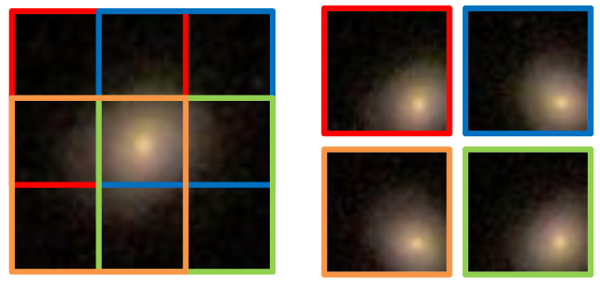
\includegraphics[width=0.7\textwidth]{zoo.png}
				\caption{S. Dieleman's cropped images for the galaxy zoo challenge\cite{zoo}}
				\label{fig:zooimage}
				\end{figure}
				\begin{figure}[H]
					\centering
						\begin{tabular}{c c c c}
						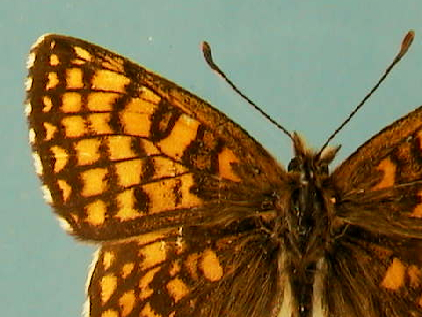
\includegraphics[width=0.2\textwidth]{Melitaea-athalia-08-01.jpg} &
						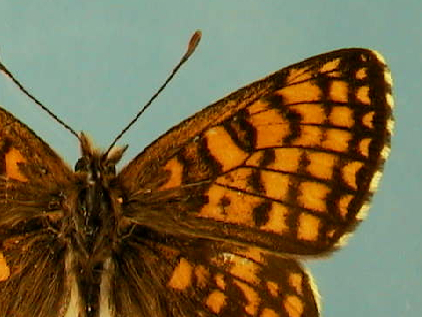
\includegraphics[width=0.2\textwidth]{Melitaea-athalia-08-02.jpg} &
						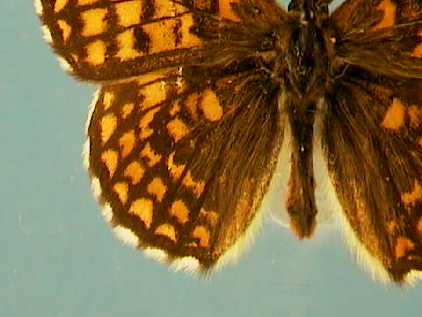
\includegraphics[width=0.2\textwidth]{Melitaea-athalia-08-03.jpg}&
						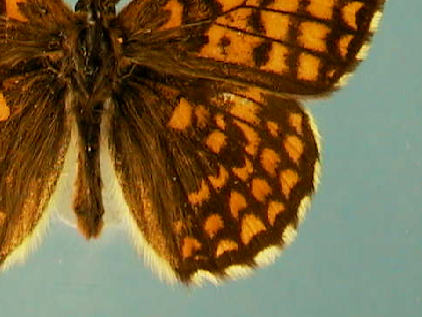
\includegraphics[width=0.2\textwidth]{Melitaea-athalia-08-04.jpg}
						\end{tabular} 
				\caption{An example of over cropping}
				\label{fig:translation}
				\end{figure}
				\item \textbf{Reflections and Rotations}. The use of these augmentations requires consideration of the data set, `does the image still make sense after such a transformation' should be asked before any transformation is made. Flowers for example are unlikely to be seen upside down hence only horizontal reflections are used\cite{imagenet} where as images of galaxies are invariant to rotations and flips\cite{zoo}. Butterflies for example are invariant to reflections about the $y$ axis due to their symmetry\cite{symmetry}.
				\begin{figure}[H]
					\centering
						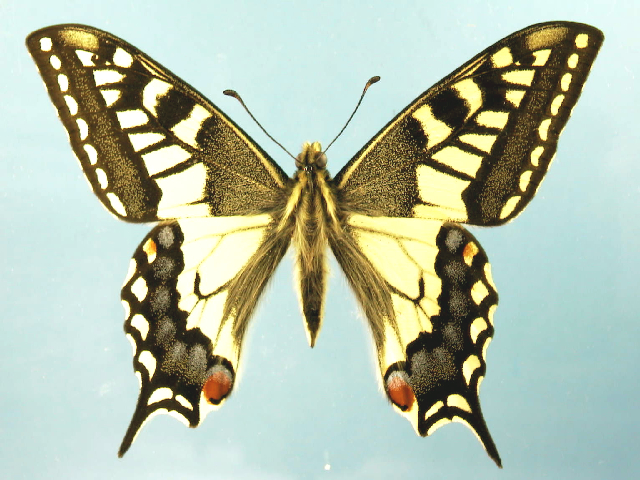
\includegraphics[width=0.4\textwidth]{Papilio-machaon-09.jpg} 
						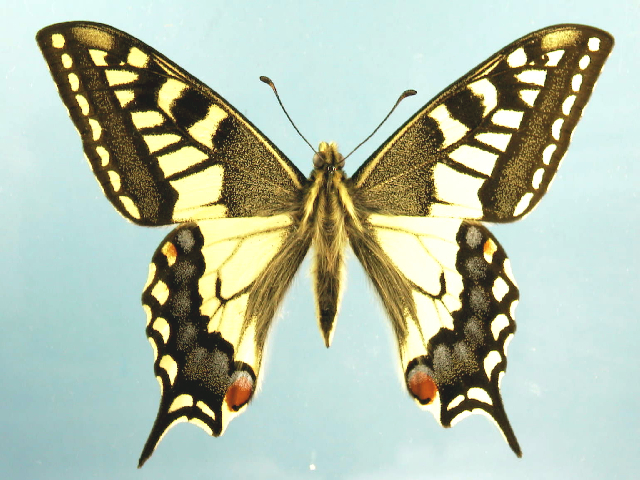
\includegraphics[width=0.4\textwidth]{Papilio-machaon-09-flip.jpg} 
				\caption{Images vertically reflected}
				\label{fig:reflected}
				\end{figure}
			\end{itemize}
			
			

%% =======================================================================%%
%%                                                                              Conclusion
%% =======================================================================%%

	\section{Conclusion}
		The image processing pipeline will be developed in modules and each module will be developed in stages, beginning with the first iteration of the segmentation module. This first iteration will be developed with a GrabCut algorithm with a manually set bounding box. The bounding box will be decided using the method of foreground intersection as previously discussed. Time permitting the segmentation module will then be improved to make use of BiCos.\\
		
		\noindent The classification module will take in as input the resultant foreground from the segmentation module and aim to return a classification. A worrying dependency on a vast amount of training data is present in the use of convolutional neural networks. Given only 5 to 10 images per class, even with methods such as dropout\cite{dropout} and data augmentation techniques (see section \ref{subsec:overfitting}) to increase the training set size\cite{zoo}, over fitting is still a real possibility. However an advantage the butterfly images have over these larger data sets is uniformity, this alone has convinced me to at least try and use convolutional neural networks as a possible core for the classification module, so potentially at a later stage of the project such a network can be built, allowing for an alternative comparative method. Initially I will implement a bag of words approach in order to classify the butterflies, using the advancement of spatial pyramids. In parallel I will attempt to build a $k$ nearest neighbour classifier, its simplicity and similarity to current technology\cite{DAISY} lends it well to use as a benchmark for progress.\\
		\subsection{Testing}

			\noindent In order to properly test and compare the different models which have been previously discussed, a thorough frame work must be in place. $k$ fold cross validation splits the dataset $D:=(x_1,...,x_n)$ into $k$ equal sized sets $(D_1,...,D_k)$. Training round $i$ uses the subset of data $D_i$ as a validation set and $D\setminus D_i$ is used to train the model, so each model is trained and tested for a total of $k$ rounds. Letting $E(m,i)$ be the error of model $m$ trained on data set $D\setminus D_i$ and validated on set $D_i$, we then define the error of the model as $\epsilon_m := \frac{\sum_{i=1}^{k} E(m,i)}{k}$, the average error over all rounds. Given that some classes only contain 5 image samples and the desire to have at least one sample from each species of butterfly in any validation set, the natural choice for $k$ is 5. This leave $\sim$80\% of the images for training and 20\% for validation, to increase the amount of training data we are able to use I propose the use of a random sub sample cross validation inspired technique instead. This is a similar method to $k$ fold cross validation except the validation set $V_i$ is a random sample of 1 image from each species and perform 5 rounds of testing per model, training in round $i$ on the set $D\setminus V_i$ and defining the model error as the average over all $i$.

%% =======================================================================%%
%%                                                                              Extension
%% =======================================================================%%
	
	\newpage
	\section{Extensions}
		A bag of words approach with spatial pyramids could be adapted, namely in the method chosen to breakdown the image into subregions. Taking advantage of the radial breakup of patterns\cite{butterfly} on a butterflies wings we could experiment with a region system similar to that in figure \ref{fig:radial}. DAISY converts images from Cartesian to polar co-ordinates\cite{DAISY} as a pre-processing stage to classification, this could also be done with our programme. Alternative a log-polar transformation could be made, this method has been used previously\cite{logpolar} in order to achieve rotation invariance as rotated images manifest as column shifts in the log-polar domain and scale differences can be mitigated by using a fixed size in the log-polar domain.
		\begin{figure}[H]
			\centering
				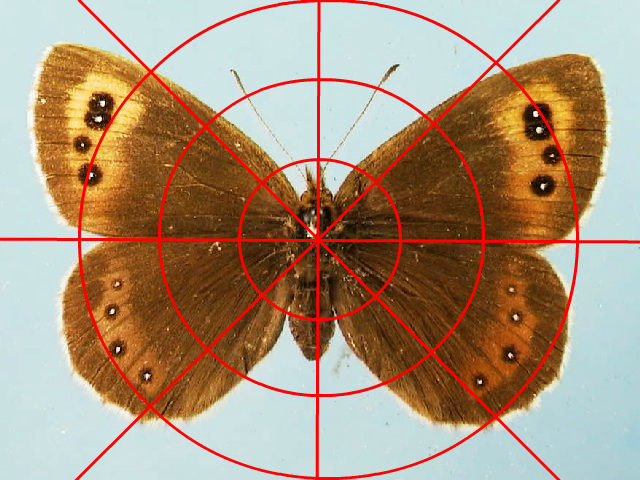
\includegraphics[width=0.4\textwidth]{Erebia-aethiops-08-radial.jpg} 
			\caption{Potential new gridded system}
			\label{fig:radial}
		\end{figure}

%% =======================================================================%%
%%                                                                              Work Plan
%% =======================================================================%%
	
	\section{Work Plan}
	Work will progress in 2 week periods as outline below (gantt chart provided in figure \ref{fig:gantt}):
		\begin{itemize}
			\item \textbf{June 01 - June 14} First iteration of segmentation module complete
			\item \textbf{June 15 - June 28} Begin iteration of classification module complete
			\item \textbf{June 29 - July 12} Complete Classification module and user interface
			\item \textbf{July 13 - July 26} Make final improvements to both modules
			\item \textbf{July 27 - September 5} Complete final report
		\end{itemize}

		\begin{figure}[H]
		\center
		\begin{ganttchart}[vgrid, hgrid style/.style=red,x unit=15mm,]{1}{9}
			\gantttitle{Project Work Plan}{9} \\
			\gantttitlelist{1,...,9}{1} \\
			\ganttbar{Segmentation module}{1}{2}
			\ganttbar{}{7}{8} \ganttnewline[thick, blue]
			\ganttbar{Classification module}{3}{5}
			\ganttbar{}{7}{8} \ganttnewline[thick, blue]
			\ganttbar {User interface}{5}{6}  \ganttnewline[thick, blue]
			\ganttbar {Final report}{9}{9}
		\end{ganttchart}

		\caption{Sections of the project being worked on each week}
		\label{fig:gantt}
		\end{figure}

%% =======================================================================%%
%%                                                                                 Work Plan
%% =======================================================================%%

%% =======================================================================%%
%%                                                                                Bibliography                                                                      %%
%% =======================================================================%%
\newpage
\bibliographystyle{plain}
\begin{thebibliography}{2}
	%\bibitem{key}
	%	author,
	%	\emph{title}.
	%	publisher, country,
	%	edition,
	%	date.
	\bibitem{nature}
		Time to automate identification.
		In \emph{NATURE},
		Vol 467,
		9 September 2010.

	\bibitem{logpolar}
		M. K. Bhowmik, D. Bhattacharjee, M. Nasipuri, M. Kundu, D. K. Basu 
		\emph{Classification of Log-Polar-Visual Eigenfaces using Multilayer Perceptron}
	\bibitem{ND}
		Y. Y. Boykov and M. P. Jolly.
		Interactive Graph Cuts for Optimal Boundary \& Region Segmentation of Objects in N-D
		In \emph{ICCV}
		2001
	\bibitem{chai}
		Y. Chai
		\emph{Recognition between a Large Number of Flower Species}
		2011
	\bibitem{bicos}
		Y. Chai, V Lempitsly, A. Zisserman.
		BiCoS: A Bi-level Co-Segmentation Method for Image Classification. 
		In \emph{ICCV},
		2011.
	\bibitem{felz}
		P. F. Felzenszwalb and D. P. Huttenlocher.
		Efficient Graph-Based Image Segmentation.
		\emph{International Journal of Computer Vision}
		59(2),
		2004
	\bibitem{dropout}
		G. E. Hinton, N. Srivastava, A. Krizhevsky, I. Sutskever and R. R. Salakhutdinov.
		Improving neural networks by preventing co-adaptation of feature detectors.
		\emph{arXiv preprint arXiv:1207.0580},
		2012
	\bibitem{imagenet}
		A. Krizhevsky, I. Sutskever and G. E. Hinton
		ImageNet Classification with Deep Convolutional Neural Networks.
		In \emph{NIPS},
		2012
	\bibitem{pyramid}
		 S. Lazebnik, C. Schmid, and J. Ponce.
		 Beyond bags of features: Spatial pyramid matching for recognizing natural scene categories.
		 In \emph{CVPR},
		 2006.
	\bibitem{sift}
		D. G. Lowe.
		Object recognition from local scale-invariant features.
		In \emph{ICCV},
		1999
	\bibitem{lucas}
		S.M. Lucas.
		Face recognition with the continuous n-tuple classifier.
		In \emph{CLARK, A.F., Ed}
		Proceedings of the English British Machine Vision Conference.
		British Machine Vision Association, pp. 222-231.
	\bibitem{book}
		Edited by N. MacLeod.
		Automated Taxon Identification in Systematics.
		In \emph{The Systematics Association},
		Special Volume Series 74
	\bibitem{vis}
		T. Malisiewicz and A. A. Efros.
		Improving spatial support for objects via multiple segmentations.
		In \emph{BMVC},
		2007
	\bibitem{butterfly}
		H. F. Nijhout.
		Elements of Butterfly Wing Patterns.
		\emph{Journal of Experimental Zoology (MOL DEV EVOL) 291:213-225},
		2001.
	\bibitem{symmetry}
		H. F. Nijhout.
		Symmetry systems and compartments in Lepidopteran wings: the evolution of a patterning mechanism.
		In \emph{Development}.
		1994.
	\bibitem{vocab}
		M-E. Nilsback and A. Zisserman.
		A Visual Vocabulary for Flower Classification
		In \emph{CVPR},
		2006
	\bibitem{deeper}
		 M-E. Nilsback and A. Zisserman.
		 Delving deeper into the whorl of flower segmentation.
		 In \emph{Image and Vision Computing},
		 2009.
	\bibitem{overview}
		M. A. O'Neil.
		\emph{DAISY: A Practical Tool for Automated Species Identification}.
	\bibitem{science}
		S. Reed
		Pushing DAISY
		In \emph{SCIENCE},
		Vol 328,
		25 June 2010.
	\bibitem{grabcut}
		C. Rother, V. Kolmogorov and A. Blake
		``GrabCut''  Interactive Foreground Extraction using Iterated Graph Cuts
		\emph{ACM Trans. Graph.},
		23(3),
		2004
	\bibitem{mr8}
		M. Varma and A. Zisserman.
		Classifying images of materials: Achieving viewpoint and illumination independence.
		In \emph{Proc. ECCV}
		volume 3,
		pages 255-271.
		Springer-Verlag,
		May 2002.
	\bibitem{DAISY}
		A. T. Watson, M. A. O'Neil and J. Kitching.
		Automated identification of live moths (Macrolepidoptera).
		1997.
	%%%%%%%%%%%%%%%%%%%%%%%%%%%%%%%%%%%%%%%%%%%%%%%%%%%%%

	\bibitem{zoo}
		\texttt{http://benanne.github.io/2014/04/05/galaxy-zoo.html}
	\bibitem{robot}
		\texttt{http://www.robots.ox.ac.uk:5000/$\sim$vgg/research/flowers\_demo/index.html}
	\bibitem{dice}
		\texttt{http://www.tumblingdice.co.uk/daisy/faq}
	\bibitem{oxford102}
		\texttt{http://www.robots.ox.ac.uk/$\sim$vgg/data/flowers/102/index.html}
	\bibitem{imagenetsite}
		\texttt{http://image-net.org/challenges/LSVRC/2010/index}
\end{thebibliography}	

%% End of document...WAHEY!
\end{document}

